\documentclass[a4paper,twoside]{article}
\usepackage[T1]{fontenc}
\usepackage[bahasa]{babel}
\usepackage{graphicx}
\usepackage{graphics}
\usepackage{float}
\usepackage[cm]{fullpage}
\pagestyle{myheadings}
\usepackage{etoolbox}
\usepackage{setspace} 
\usepackage{lipsum} 
\usepackage{listings}
\setlength{\headsep}{30pt}
\usepackage[inner=2cm,outer=2.5cm,top=2.5cm,bottom=2cm]{geometry} %margin
% \pagestyle{empty}
\lstdefinestyle{mystyle}{
	basicstyle=\ttfamily\footnotesize,
	breakatwhitespace=false,         
	breaklines=true,                                    
	keepspaces=true,                 
	numbers=left,                    
	numbersep=5pt,                  
	showspaces=false,                
	showstringspaces=false,
	showtabs=false,                  
	tabsize=2
}
\usepackage{graphicx}
\usepackage{float}
\lstset{style=mystyle}
\usepackage{hyperref}
\hypersetup{
	colorlinks=true,
	linkcolor=blue,
	filecolor=magenta,      
	urlcolor=cyan,
	pdftitle={Overleaf Example},
	pdfpagemode=FullScreen,
}


\makeatletter
\renewcommand{\@maketitle} {\begin{center} {\LARGE \textbf{ \textsc{\@title}} \par} \bigskip {\large \textbf{\textsc{\@author}} }\end{center} }
\renewcommand{\thispagestyle}[1]{}
\markright{\textbf{\textsc{Laporan Perkembangan Pengerjaan Skripsi\textemdash Sem. Genap 2015/2016}}}

\onehalfspacing
 
\begin{document}

\title{\@judultopik}
\author{\nama \textendash \@npm} 

%ISILAH DATA BERIKUT INI:
\newcommand{\nama}{Reinalta Sugianto}
\newcommand{\@npm}{2017730035}
\newcommand{\tanggal}{13/12/2021} %Tanggal pembuatan dokumen
\newcommand{\@judultopik}{Perekaman Kehadiran Daring Otomatis} % Judul/topik anda
\newcommand{\kodetopik}{PAN5191}
\newcommand{\jumpemb}{1} % Jumlah pembimbing, 1 atau 2
\newcommand{\pembA}{Pascal Alfadian Nugroho}
\newcommand{\pembB}{-}
\newcommand{\semesterPertama}{51 - Ganjil 21/22} % semester pertama kali topik diambil, angka 1 dimulai dari sem Ganjil 96/97
\newcommand{\lamaSkripsi}{1} % Jumlah semester untuk mengerjakan skripsi s.d. dokumen ini dibuat
\newcommand{\kulPertama}{Skripsi 1} % Kuliah dimana topik ini diambil pertama kali
\newcommand{\tipePR}{B} % tipe progress report :
% A : dokumen pendukung untuk pengambilan ke-2 di Skripsi 1
% B : dokumen untuk reviewer pada presentasi dan review Skripsi 1
% C : dokumen pendukung untuk pengambilan ke-2 di Skripsi 2

% Dokumen hasil template ini harus dicetak bolak-balik !!!!

\maketitle

\pagenumbering{arabic}

\section{Data Skripsi} %TIDAK PERLU MENGUBAH BAGIAN INI !!!
Pembimbing utama/tunggal: {\bf \pembA}\\
Pembimbing pendamping: {\bf \pembB}\\
Kode Topik : {\bf \kodetopik}\\
Topik ini sudah dikerjakan selama : {\bf \lamaSkripsi} semester\\
Pengambilan pertama kali topik ini pada : Semester {\bf \semesterPertama} \\
Pengambilan pertama kali topik ini di kuliah : {\bf \kulPertama} \\
Tipe Laporan : {\bf \tipePR} -
\ifdefstring{\tipePR}{A}{
			Dokumen pendukung untuk {\BF pengambilan ke-2 di Skripsi 1} }
		{
		\ifdefstring{\tipePR}{B} {
				Dokumen untuk reviewer pada presentasi dan {\bf review Skripsi 1}}
			{	Dokumen pendukung untuk {\bf pengambilan ke-2 di Skripsi 2}}
		}
		
\section{Latar Belakang}
Perkuliahan di UNPAR biasanya membutuhkan perekaman kehadiran untuk mengetahui kehadiran mahasiswa dan dosen, bagi mahasiswa UNPAR perekaman kehadiran biasanya dilakukan dengan melakukan tanda tangan pada daftar kehadiran atau dicatat langsung oleh dosen yang memanggil mahasiswanya, sedangkan bagi dosen UNPAR perekaman kehadiran dilakukan dengan menggunakan  \textit{fingerprint}. Perekaman kehadiran diperkirakan membutuhkan waktu sekitar kurang dari 5 detik.

Pada tahun 2020 terjadi pandemi Covid-19 di seluruh negara. Pandemi Covid-19 masuk ke Indonesia pada awal bulan Maret tahun 2020. Covid-19 adalah penyakit yang disebabkan oleh virus \textit{severe acute respiratory syndrome coronavirus 2} (SARS-CoV-2). Penularan virus Covid-19 terjadi saat seseorang menyentuh barang yang sudah terkontaminasi oleh droplet orang yang terkena virus Covid-19 atau terkena droplet orang lain saat berinteraksi langsung dengan orang yang terkena virus Covid-19.  Akibat pandemi Covid-19 yang dapat menular ini, maka hampir seluruh kegiatan di Indonesia dilakukan secara daring untuk mengurangi interaksi orang secara langsung yang dapat meningkatkan angka penularan virus tersebut. 

Pembelajaran secara daring diberlakukan oleh UNPAR di akhir bulan Maret untuk seluruh kegiatan perkuliahan demi mencegah penularan virus Covid-19. Akibat diberlakukannya pembelajaran secara daring, maka perekaman kehadiran di UNPAR dilakukan dengan menggunakan aplikasi atau situs web milik UNPAR. Cara perekaman kehadiran secara daring di UNPAR ini mumbutuhkan waktu lebih agar dapat tercatat perekaman kehadirannya, karena butuh waktu untuk membuka situs web serta perlu memasukan \textit{email} dan \textit{password} hingga akhirnya melakukan perekaman kehadiran. 

Selenium adalah \textit{open-source} \textit{framework} pengujian otomatisasi untuk aplikasi web. WebDriver menggunakan API otomatisasi \textit{browser} yang disediakan oleh vendor \textit{browser} untuk mengontrol \textit{browser} dan melakukan pengujian. API WebDriver ini seolah-olah membuat pengguna secara langsung mengoperasi \textit{browser}, padahal dijalankan secara otomatis langsung oleh \textit{API} WebDriver tersebut. Selenium WebDriver adalah sebuah \textit{tools} yang berguna untuk melakukan otomatisasi terhadap web pada \textit{browser}. Selenium WebDriver ini tersedia untuk bahasa pemrograman Ruby, Java, Python, C\#, dan JavaScript. Pembuatan Perekaman kehadiran daring otomatis ini akan menggunakan Selenium WebDriver dengan bahasa pemrograman Python.  

Pada skripsi ini, akan dibuat sebuah perangkat lunak yang dapat melakukan perekaman kehadiran otomatis dengan sistem menerima rangsangan satu ``klik'' sehingga dapat melakukan hal-hal berikut :
\begin{enumerate}
	\item Membuka peramban.
	\item Membuka situs web perekaman kehadiran.
	\item Mengisi dan \textit{login} dengan \textit{username} serta \textit{password} yang diambil dari file konfigurasi.
	\item Melakukan rekam kehadiran.
\end{enumerate} 
perangkat lunak ini bertujuan agar mahasiswa dan dosen dapat melakukan perekaman kehadiran secara online dengan lebih mudah serta mengurangi waktu yang dibutuhkan untuk berinteraksi dengan aplikasi atau situs web dan bukan untuk mempercepat waktu agar kehadiran terekam, sehingga membuat waktu perekaman kehadiran secara daring dapat menyamai waktu perekaman kehadiran secara luring. 

\section{Rumusan Masalah}
Rumusan masalah yang akan dibahas di skripsi ini adalah sebagai berikut :
\begin{itemize}
	\item Bagaimana cara membangun program Perekaman Kehadiran Daring Otomatis?
	\item Bagaimana cara mengurangi waktu interaksi dengan aplikasi atau situs web untuk merekam kehadiran?
\end{itemize}

\section{Tujuan}
Tujuan yang ingin dicapai dari penulisan skripsi ini sebagai berikut :
\begin{itemize}
	\item Membangun program menggunakan Selenium WebDriver.
	\item Membuat program yang mampu menerima rangsangan satu tombol untuk melakukan beberapa hal menggunakan Selenium.
\end{itemize}

\section{Detail Perkembangan Pengerjaan Skripsi}
Detail bagian pekerjaan skripsi sesuai dengan rencan kerja/laporan perkembangan terkahir :
	\begin{enumerate}
		\item \textbf{Melakukan studi literatur mengenai Selenium WebDriver.}\\
		{\bf Status :} Ada sejak rencana kerja skripsi.\\
		{\bf Hasil :} Studi literatur mengenai Selenium WebDriver dilakukan dengan cara membaca situs web resmi Selenium Webdriver, situs-situs pembelajaran terkait, dan menonton video
		pembelajaran dari youtube. Selenium adalah \textit{open-source} \textit{framework} pengujian otomatisasi untuk aplikasi web. Selenium ini adalah WebDriver yang merupakan sebuah \textit{interface} untuk menulis suatu instruksi yang dapat dijalankan secara otomatis dan bergantian pada \textit{browser}.  Selenium WebDriver adalah sebuah \textit{tools} yang berguna untuk melakukan otomatisasi terhadap web pada \textit{browser}. Selenium WebDriver menggunakan API otomatisasi \textit{browser} yang disediakan oleh vendor \textit{browser} untuk mengontrol \textit{browser} dan melakukan pengujian. API WebDriver ini seolah-olah membuat pengguna secara langsung mengoperasi \textit{browser}, padahal dijalankan secara otomatis langsung oleh \textit{API} WebDriver tersebut. Selenium WebDriver ini tersedia untuk bahasa pemrograman Ruby, Java, Python, C\#, dan JavaScript. Selenium WebDriver memiliki berbagai fungsi, yaitu Navigasi \textit{Browser} serta Menemukan elemen.
		Salah satu teknik mendasar untuk dipelajari saat menggunakan WebDriver adalah cara menemukan elemen di halaman web. WebDriver menyediakan berbagai cara untuk menemukan elemen, terdapat delapan strategi menemukan lokasi elemen yang berbeda di WebDriver:
		\begin{enumerate}
			\item Id : Menemukan elemen yang atribut ID-nya cocok dengan nilai pencarian.
			\item \textit{Class name}: Menemukan elemen yang nama kelasnya berisi nilai pencarian.	
			\item \textit{CSS selector}: Menemukan elemen yang cocok dengan pemilihan \textit{Cascading Style Sheets} (CSS). Pemilihan pada CSS adalah pola yang digunakan untuk memilih elemen dengan \textit{style} yang diinginkan.
			\item \textit{Name}: Menemukan elemen yang atribut \textit{name} yang cocok dengan nilai pencarian.
			\item Link text: Menemukan elemen \textit{link} yang teksnya terlihat cocok dengan nilai pencarian.
			\item Partial link text: Menemukan elemen \textit{link} yang teksnya terlihat berisi nilai pencarian. Jika beberapa elemen cocok, hanya yang pertama yang akan dipilih.
			\item Tag name: Menemukan elemen yang nama tagnya cocok dengan nilai pencarian.
			\item XPath: Menemukan elemen yang cocok dengan ekspresi \textit{XML Path Language} (XPath).
		\end{enumerate}
		WebDriver secara umum dapat dikatakan memiliki API pemblokiran, karena ini adalah \textit{library} di luar proses yang menginstruksikan browser apa yang harus dilakukan dan karena platform web secara intrinsik memiliki sifat asinkron atau tidak dilakukan secara \textit{real time}, maka WebDriver tidak melacak status \textit{Document Object Model} (DOM) yang aktif dan \textit{real time}, sehingga selenium memiliki fungsi \textit{waits} untuk mengatasi hal tersebut. Berikut ini adalah beberapa fungsi \textit{Waits} pada selenium.
		\begin{enumerate}
			\item Implicit wait: memberi tahu WebDriver untuk melakukan polling DOM selama jangka waktu tertentu ketika mencoba menemukan elemen. Pengaturan awalnya adalah 0 detik, artinya dinonaktifkan. Setelah disetel, maka \textit{wait implicit} disetel untuk masa pakai sesi yang sudah disetel.
			\item Explicit wait: mengizinkan kode untuk menghentikan eksekusi program, atau membekukan \textit{thread}, hingga suatu kondisi dapat teratasi. Kondisi ini dipanggil dengan frekuensi tertentu sampai batas waktu tunggu terlewati.
		\end{enumerate}
		Selenium Webdriver sudah didokumentasikan pada Bab 2 Dasar Teori.
		
		\item \textbf{Mempelajari bahasa pemrograman python.}\\
		{\bf Status :} Ada sejak rencana kerja skripsi.\\
		{\bf Hasil :} Bahasa pemrograman dengan python dipelajari secara mandiri dengan cara membaca situs-situs pembelajaran terkait, menonton video pembelajaran dari youtube, dan mengambil mata kuliah Pengantar Penambangan Data dengan Python yang melakukan praktek dan eksplorasi menggunakan bahasa pemrograman python.

		\item \textbf{Mempelajari cara menggunakan Selenium.}\\
		{\bf Status :} Ada sejak rencana kerja skripsi.\\
		{\bf Hasil :} Mempelajari cara menggunakan selenium dengan studi literatur tentang selenium webdriver terlebih dahulu, lalu melakukan eksplorasi menggunakan selenium tersebut secara langsung menggunakan bahasa pemrograman python terhadap situs web Portal Mahasiswa UNPAR. Berikut ini merupakan kode program hasil dari ekplorasi percobaan menggunakan selenium.
		\begin{lstlisting}[language=python, caption=Eksplorasi kode Program menggunakan Selenium]
	import config_file as cfg
	from selenium import webdriver
	from selenium.webdriver.common.by import By
	from selenium.webdriver.support import expected_conditions as EC
	from selenium.webdriver.support.ui import WebDriverWait
	driver = webdriver.Chrome(executable_path='D:\Skripsi\python\chromedriver.exe')
	driver.maximize_window()
	portal = driver.get("https://studentportal.unpar.ac.id/")
	btnIn = driver.find_element(By.CSS_SELECTOR,"#login-button").click()
	inputEmail= driver.find_element(By.CSS_SELECTOR,"#username").send_keys(cfg.drivers_config["email"])
	btnNext = driver.find_element(By.CSS_SELECTOR, "#next_login").click()
	inputPassword = WebDriverWait(driver, 10).until(EC.element_to_be_clickable((By.CSS_SELECTOR,"#password")))
	inputPassword.click()
	inputPassword.send_keys(cfg.drivers_config["pass"])
	btnLogin = driver.find_element(By.CSS_SELECTOR,"#appPass > div.login__form > button").click()\end{lstlisting}
	Pada contoh eksplorasi kode program di atas akan dijelaskan perbaris sebagai berikut:
	\begin{enumerate}
		\item Baris 1: melakukan import file konfigurasi yang telah dibuat.
		\item Baris 2: melakukan import webdriver dari selenium yang berguna untuk membuka \textit{browser}.
		\item Baris 3: melakukan import By untuk menemukan elemen yang ingin dicari.
		\item Baris 4: melakukan import expected\_conditions yang berguna mengharapkan suatu kondisi dapat terjadi.
		\item Baris 5: melakukan import WebDriverWait berguna untuk fungsi \textit{Waits} pada selenium untuk memberi waktu melakukan suatu perintah.
		\item Baris 6: memanggil webdriver yang ingin digunakan, yaitu Google Chrome dan diisi letak file chromedriver.exe disimpan.
		\item Baris 7: untuk memberi perintah \textit{fullscreen} pada \textit{browser} Google Chrome.
		\item Baris 8: \textit{String} portal menggunakan \textit{method get} yang berguna untuk menuju situs web Portal Mahasiswa UNPAR.
		\item Baris 9: \textit{String} btnIn untuk menemukan elemen dari sebuah tombol menggunakan \textit{CSS selector} dengan nama ``\#login-button'', lalu menggunakan \textit{method click} untuk menekan tombol tersebut secara otomatis.  
		\item Baris 10: \textit{String} inputEmail untuk menemukan elemen dari sebuah \textit{input teks} menggunakan \textit{CSS selector} dengan nama ``\#username'', lalu menggunakan \textit{method send\_keys} untuk memasukan email mahasiswa yang sudah dibuat di file konfigurasi untuk dipanggil.
		\item Baris 11: \textit{String} btnNext untuk menemukan elemen dari sebuah tombol menggunakan \textit{CSS selector} dengan nama ``\#next\_login'', lalu menggunakan \textit{method click} untuk menekan tombol tersebut secara otomatis.
		\item Baris 12: \textit{String} inputPassword memanggil fungsi \textit{waits} selama 10 detik untuk menunggu elemen yang dicari berdasarkan \textit{CSS selector} dengan nama ``\#password'' ini dapat ditekan.
		\item Baris 13: Memerintahkan untuk menekan elemen yang sudah dicari pada baris 12.
		\item Baris 14: Memerintahkan untuk memasukan \textit{password} yang sudah dibuat di file konfigurasi untuk dipanggil.
		\item Baris 15: \textit{String} btnLogin untuk menemukan elemen dari sebuah tombol \textit{login} menggunakan \textit{CSS selector}, lalu menekannya.
	\end{enumerate}
	
		\item \textbf{Melakukan survei ke mahasiswa dan dosen Teknik Informatika Universitas Katolik Parahyangan untuk mengetahui berapa lama waktu yang dibutuhkan untuk melakukan absensi secara daring dan luring.}\\
		{\bf Status :} Baru ditambahkan pada semester ini.\\
		{\bf Hasil :} Hasil survei telah ditulis dan dianalisis pada Bab 3. Survei dilakukan dengan menyebarkan \textit{Google Form} kepada mahasiswa dan dosen Teknik Informatika Universitas Katolik Parahyangan. Survei ini bertujuan untuk mengetahui waktu yang dibutuhkan untuk melakukan absensi secara daring dan luring. 
		\subsection{Hasil Survei Mahasiswa}
		Berdasarkan hasil survei yang telah diterima dari 21 orang responden yang merupakan mahasiswa Teknik Informatika Universitas Katolik
		Parahyangan yang terdiri dari mahasiswa angkatan 2017 sampai 2019, dengan pertanyaan yang diajukan kepada responen dan rangkuman jawaban hasil survei sebagai berikut:
		\begin{enumerate}
			\item \textbf{Berapa detik perkiraan waktu interaksi yang Anda butuhkan untuk melakukan perekaman kehadiran daring di \url{https://studentportal.unpar.ac.id/}, mulai dari membuka \textit{browser}, lalu masuk ke \url{https://studentportal.unpar.ac.id/}, lalu mengklik tombol presensi?}
			\begin{figure}[H]
				\centering
				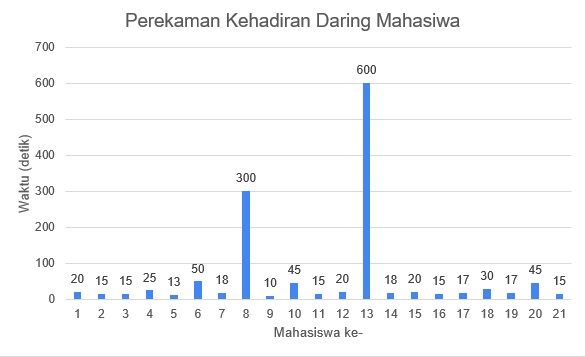
\includegraphics[scale=0.8]{Gambar/DaringMahasiswa.jpg}
				\caption{Histogram Waktu Perekaman Kehadiran Daring Mahasiswa} 
				\label{fig:DaringMahasiswa}
			\end{figure}
			Pada Gambar \ref{fig:DaringMahasiswa} merupakan visualisasi dari hasil survei mengenai lama waktu yang dibutuhkan dari 21 mahasiswa untuk melakukan perekaman kehadiran secara daring.
			Jawaban dari 21 orang responden adalah mulai dari waktu paling cepat 10 detik hingga waktu paling lama 600 detik.\\ \\
			\begin{tabular}{|p{4cm} |p{7cm}|}
				\hline
				Jumlah Responden &  Waktu Perekaman Kehadiran Daring \\ \hline     
				1 orang &  10 detik\\ \hline 
				1 orang &  13 detik\\ \hline 
				5 orang &  15 detik\\ \hline 
				2 orang &  17 detik\\ \hline 
				2 orang &  18 detik\\ \hline 
				3 orang &  20 detik\\ \hline
				1 orang &  25 detik\\ \hline 
				1 orang &  30 detik\\ \hline 
				2 orang &  45 detik\\ \hline
				1 orang &  50 detik\\ \hline 
				1 orang &  300 detik\\ \hline 
				1 orang &  600 detik\\ \hline
			\end{tabular}\\ \\
			Jika dihitung rata-rata waktu yang dibutuhkan untuk melakukan perekaman kehadiran daring bagi para mahasiswa adalah 63 detik.
			
			\item \textbf{Berapa detik perkiraan waktu interaksi yang Anda butuhkan untuk melakukan perekaman kehadiran luring menggunakan metode tanda tangan seperti pembelajaran di kelas, mulai dari mengambil kertas absen, lalu tanda tangan, lalu memberikannya ke rekan di sebelah anda?}
			\begin{figure}[H]
				\centering
				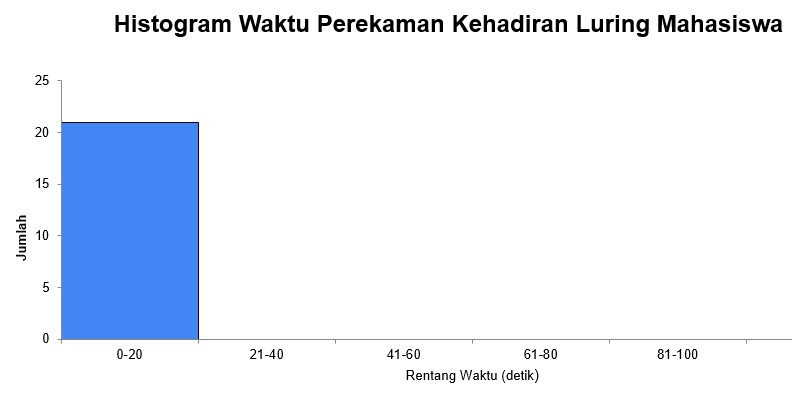
\includegraphics[scale=0.8]{Gambar/LuringMahasiswa.jpg}
				\caption{Histogram Waktu Perekaman Kehadiran Daring Mahasiswa} 
				\label{fig:LuringMahasiswa}
			\end{figure}
			Pada Gambar \ref{fig:LuringMahasiswa} merupakan visualisasi dari hasil survei mengenai lama waktu yang dibutuhkan dari 21 mahasiswa untuk melakukan perekaman kehadiran secara luring.
			Jawaban dari 21 orang responden adalah mulai dari waktu paling cepat 5 detik hingga waktu paling lama 15 detik.\\ \\
			\begin{tabular}{|p{4cm} |p{7cm}|}
				\hline
				Jumlah Responden &  Waktu Perekaman Kehadiran Luring \\ \hline     
				5 orang &  5 detik\\ \hline 
				1 orang &  6 detik\\ \hline 
				5 orang &  7 detik\\ \hline 
				2 orang &  8 detik\\ \hline 
				7 orang &  10 detik\\ \hline 
				1 orang &  15 detik\\ \hline
			\end{tabular}\\ \\
			Jika dihitung rata-rata waktu yang dibutuhkan untuk melakukan perekaman kehadiran luring bagi para mahasiswa adalah 7,95 detik.
		\end{enumerate}
		Kesimpulan dari hasil survei mahasiswa menunjukan bahwa rata-rata waktu yang dibutuhkan secara luring adalah 7,95 detik lebih cepat dibandingkan dengan rata-rata waktu yang dibutuhkan secara daring adalah waktu 63 detik
		
		\subsection{Hasil Survei Dosen}
		Berdasarkan hasil survei yang telah diterima dari 6 orang responden yang merupakan dosen Teknik Informatika Universitas Katolik Parahyangan, dengan pertanyaan yang diajukan kepada responen dan rangkuman jawaban hasil survei sebagai berikut:
		\begin{figure}[H]
			\centering
			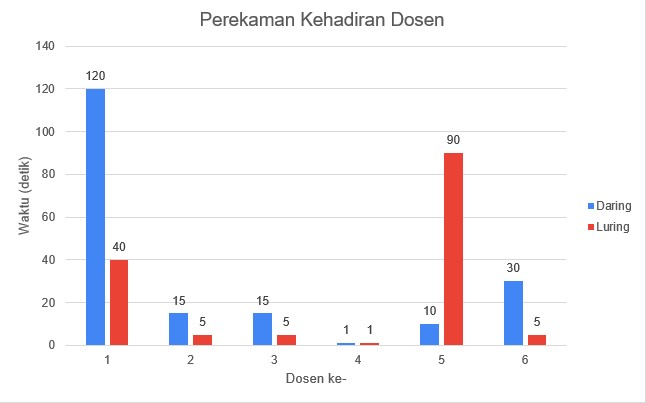
\includegraphics[scale=0.8]{Gambar/GrafikDosen.jpg}
			\caption{Histogram Perbandingan Waktu Perekaman Kehadiran Dosen} 
			\label{fig:GrafikDosen}
		\end{figure}
		Pada Gambar \ref{fig:GrafikDosen} merupakan visualisasi dari perbandingan waktu yang dibutuhkan dari 6 dosen Teknik Informatika Universitas Katolik Parahyangan. Grafik warna biru menjelaskan perekaman kehadiran secara daring dan warna merah menjelaskan perekaman kehadiran secara luring. Mayoritas menyatakan bahwa perekaman kehadiran luring lebih cepat dibandingkan daring, hanya dosen ke-4 yang menyatakan waktunya sama dan dosen ke-5 yang menyatakan waktu perekaman kehadiran daring lebih cepat dibandingkan luring.
		\begin{enumerate}
			\item \textbf{Berapa detik perkiraan waktu interaksi yang Anda butuhkan untuk melakukan perekaman kehadiran daring di \url{https://akuhadir.unpar.ac.id ?}}\\
			\begin{tabular}{|p{4cm} |p{7cm}|}
				\hline
				Jumlah Responden &  Waktu Perekaman Kehadiran Daring \\ \hline     
				1 orang &  1 detik\\ \hline 
				1 orang &  10 detik\\ \hline 
				2 orang &  15 detik\\ \hline 
				1 orang &  30 detik\\ \hline 
				1 orang &  120 detik\\ \hline 
			\end{tabular}\\ \\
			Jika dihitung rata-rata waktu yang dibutuhkan untuk melakukan perekaman kehadiran daring bagi para dosen adalah 31,83 detik.
		
			\item \textbf{Berapa detik perkiraan waktu interaksi yang Anda butuhkan untuk melakukan perekaman kehadiran luring menggunakan metode fingerprint?}\\
			\begin{tabular}{|p{4cm} |p{7cm}|}
				\hline
				Jumlah Responden &  Waktu Perekaman Kehadiran Luring \\ \hline     
				1 orang &  1 detik\\ \hline 
				3 orang &  5 detik\\ \hline 
				1 orang &  40 detik\\ \hline 
				1 orang &  90 detik\\ \hline 
			\end{tabular}\\ \\
			Jika dihitung rata-rata waktu yang dibutuhkan untuk melakukan perekaman kehadiran luring bagi para dosen adalah 24,33 detik.
		\end{enumerate}
		Kesimpulan dari hasil survei dosen menunjukan bahwa rata-rata waktu yang dibutuhkan secara luring adalah 24,33 detik lebih cepat dibandingkan dengan rata-rata waktu yang dibutuhkan secara daring adalah waktu 31,83 detik. 
		
		\item \textbf{Menganalisis web \textit{Student} Portal UNPAR.}\\
		{\bf Status :} Ada sejak rencana kerja skripsi.\\
		{\bf Hasil :} Portal Akademik Mahasiswa adalah sebuah web yang di peruntukan bagi mahasiswa dalam rangka mendapatkan informasi kegiatan akademik mulai dari registrasi, melihat jadwal kuliah dan ujian, info nilai sampai pendaftaran sidang. Portal Akademik Mahasiswa dapat diakses melalui \url{https://studentportal.unpar.ac.id/}. Portal Akademik Mahasiswa Universitas Katolik Parahyangan yang terbaru sejak 2020 sudah dapat melakukan perekaman kehadiran secara online untuk setiap mata kuliah yang diambil. Analisis pada Portal Akademik Mahasiswa yang diutamakannya adalah bagaimana alur cara melakukan absensi pada mata kuliah. Berikut ini adalah alur untuk melakukan perekaman kehadiran online melalui Portal Akademik Mahasiswa Universitas Katolik Parahyangan:
		\begin{enumerate}
			\item Melakukan akses Portal Akademik Mahasiswa yang dapat diakses melalui \url{https://studentportal.unpar.ac.id/}.
			\begin{figure}[H]
				\centering
				
\includegraphics[scale=0.225]{Gambar/halaman2019.jpg}
				\caption{Tampilan halaman awal Portal Akademik Mahasiswa} 
				\label{fig:studpor_home_2019}
			\end{figure}
			\item Menekan tombol ``Login'' yang sudah tersedia agar dapat masuk ke dalam Portal Akademik Mahasiswa, dapat dilihat pada Gambar \ref{fig:studpor_home_2019}.
			
			\item Memasukan \textit{email} mahasiswa.
			\begin{figure}[H]
				\centering
				
\includegraphics[scale=0.225]{Gambar/login.jpg}
				\caption{Tampilan halaman Portal Akademik Mahasiswa untuk memasukan \textit{email}} 
				\label{fig:login}
			\end{figure}
			\item Menekan tombol ``NEXT'' setelah memasukan \textit{email}, dapat dilihat pada Gambar \ref{fig:login}.
			
			\item Memasukan \textit{password} milik mahasiswa.
			\begin{figure}[H]
				\centering
				
\includegraphics[scale=0.225]{Gambar/pass.jpg}
				\caption{Tampilan halaman Portal Akademik Mahasiswa untuk memasukan \textit{password}} 
				\label{fig:pass}
			\end{figure}
			\item Menekan tombol ``LOGIN'' setelah memasukan \textit{password}, dapat dilihat pada Gambar \ref{fig:pass}.
			
			\item Menekan tombol ``Tutup'' jika muncul peringatan atau langsung menekan tombol berbentuk heksagon ``JADWAL \& KEHADIRAN'' jika tidak muncul peringatan.
			\begin{figure}[H]
				\centering
				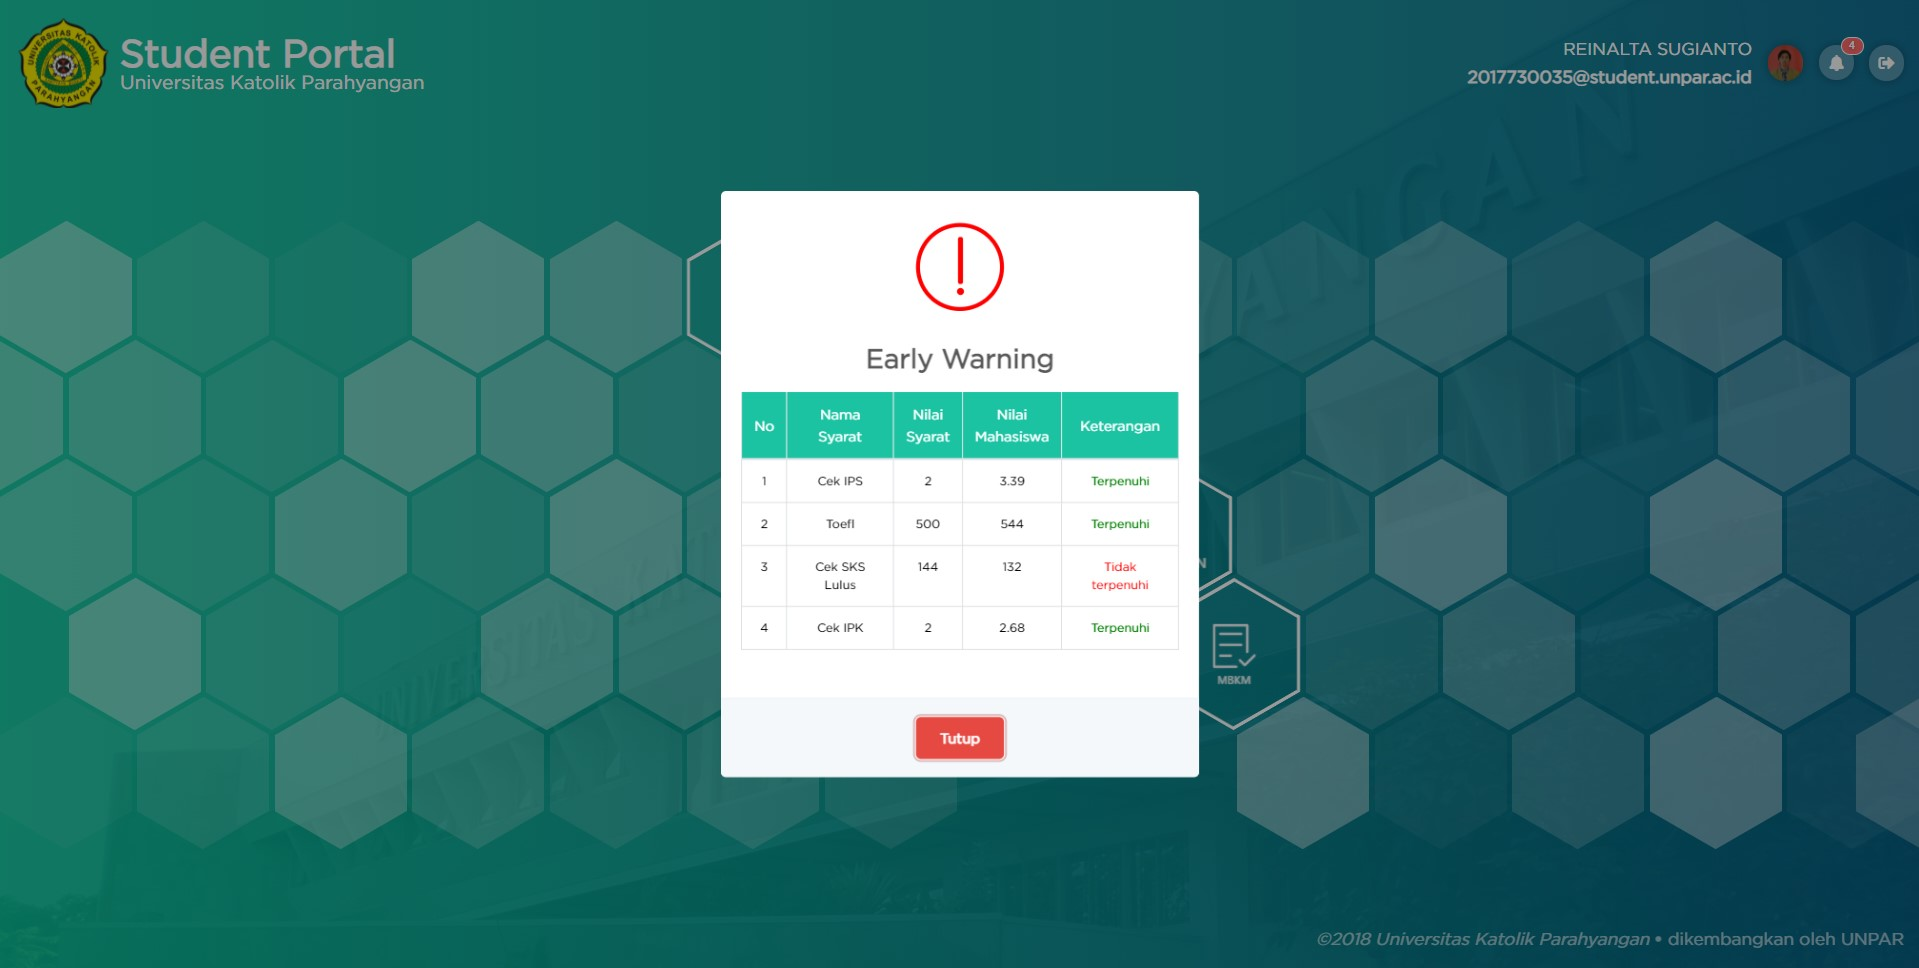
\includegraphics[scale=0.225]{Gambar/notif.jpg}
				\caption{Tampilan peringatan pada halaman Portal Akademik Mahasiswa} 
				\label{fig:notif}
			\end{figure}
			
			\begin{figure}[H]
				\centering
				
\includegraphics[scale=0.225]{Gambar/jadwal.jpg}
				\caption{Tampilan halaman Portal Akademik Mahasiswa setelah Berhasil \textit{Login}} 
				\label{fig:jadwal}
			\end{figure}
			Pada Gambar \ref{fig:notif} merupakan sebuah peringatan yang terkadang muncul menjelang berakhirnya suatu semester untuk melihat status kebutuhan mahasiswa untuk lulus, sehingga perlu menekan tombol ``Tutup'' terlebih dahulu untuk menekan tombol berbentuk heksagon ``JADWAL \& KEHADIRAN'' seperti pada Gambar \ref{fig:jadwal}. Jika tidak terjadi peringatan seperti pada  Gambar \ref{fig:notif}, maka dapat langsung menekan tombol berbentuk heksagon ``JADWAL \& KEHADIRAN'' seperti pada Gambar \ref{fig:jadwal}.
			
			\item Menekan tombol berwarna merah pada kolom bagian persensi dari tabel jadwal kehadiran mata kuliah. 
			\begin{figure}[H]
				\centering
				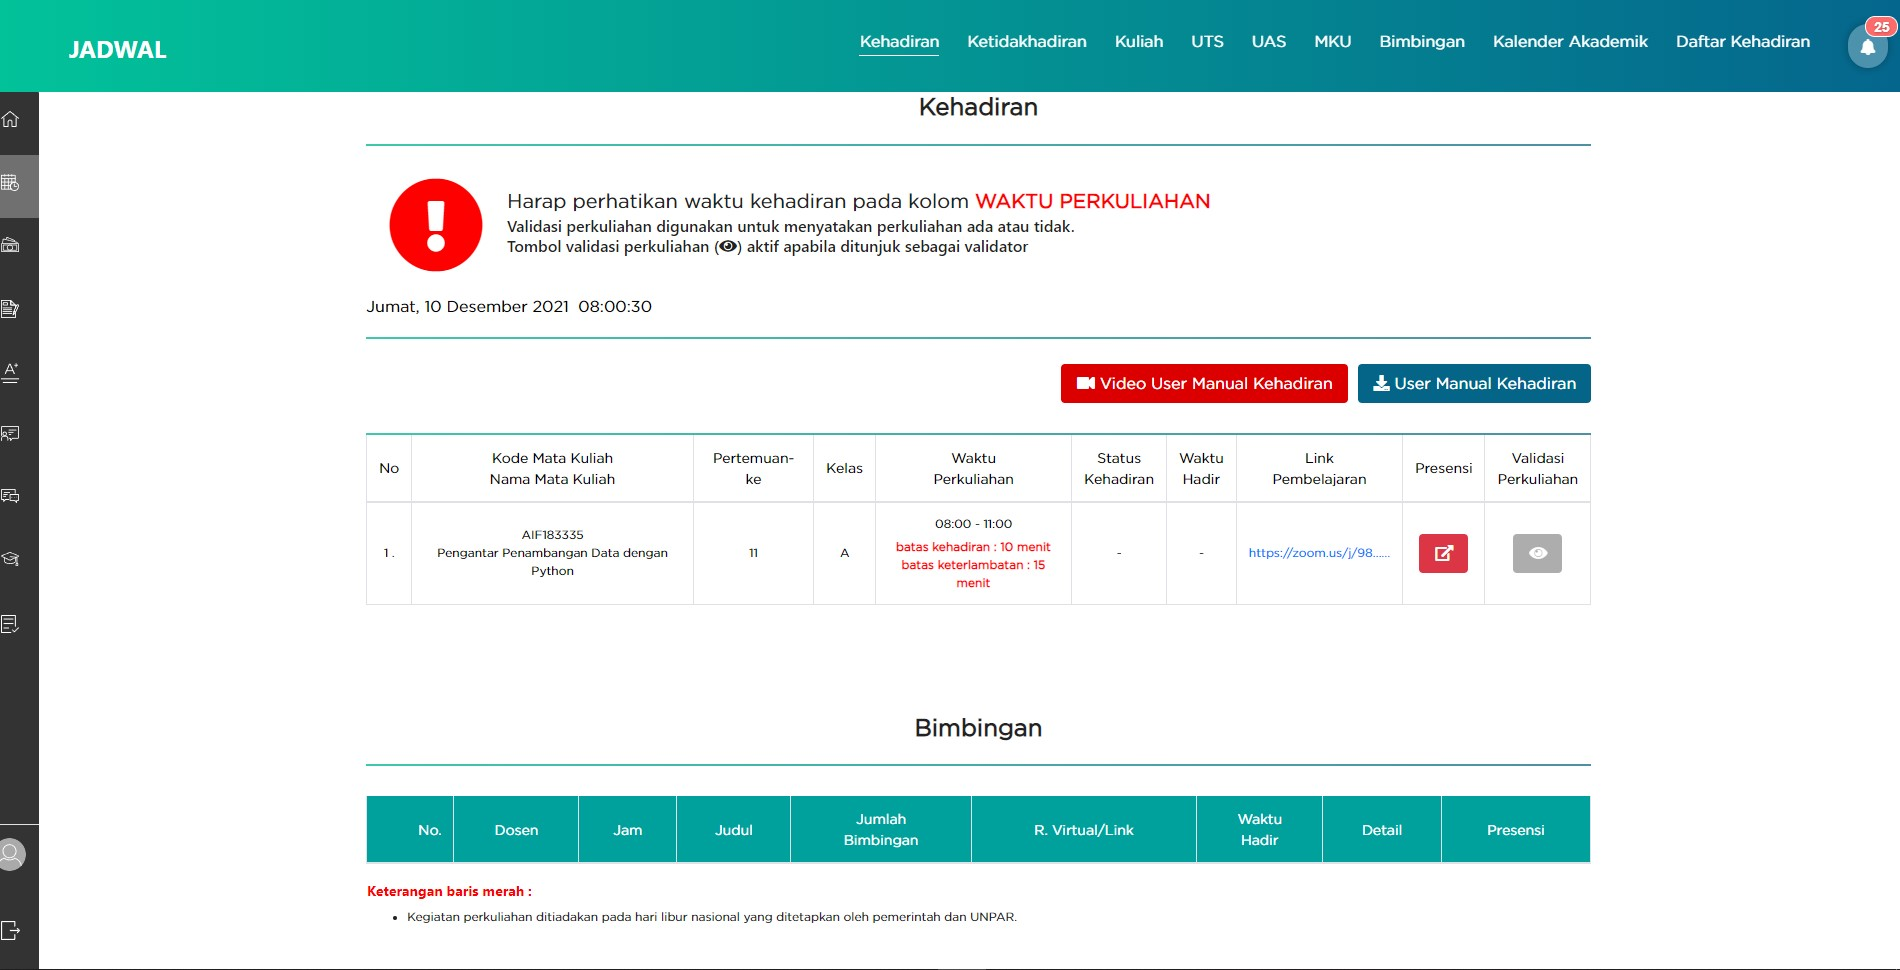
\includegraphics[scale=0.225]{Gambar/absen.jpg}
				\caption{Tampilan halaman Portal Akademik Mahasiswa untuk Melakukan Absen} 
				\label{fig:absen}
			\end{figure}
			
			\item Menekan tombol ``OK'' ketika muncul pemberitahuan setelah berhasil melakukan presensi.
			\begin{figure}[H]
				\centering
				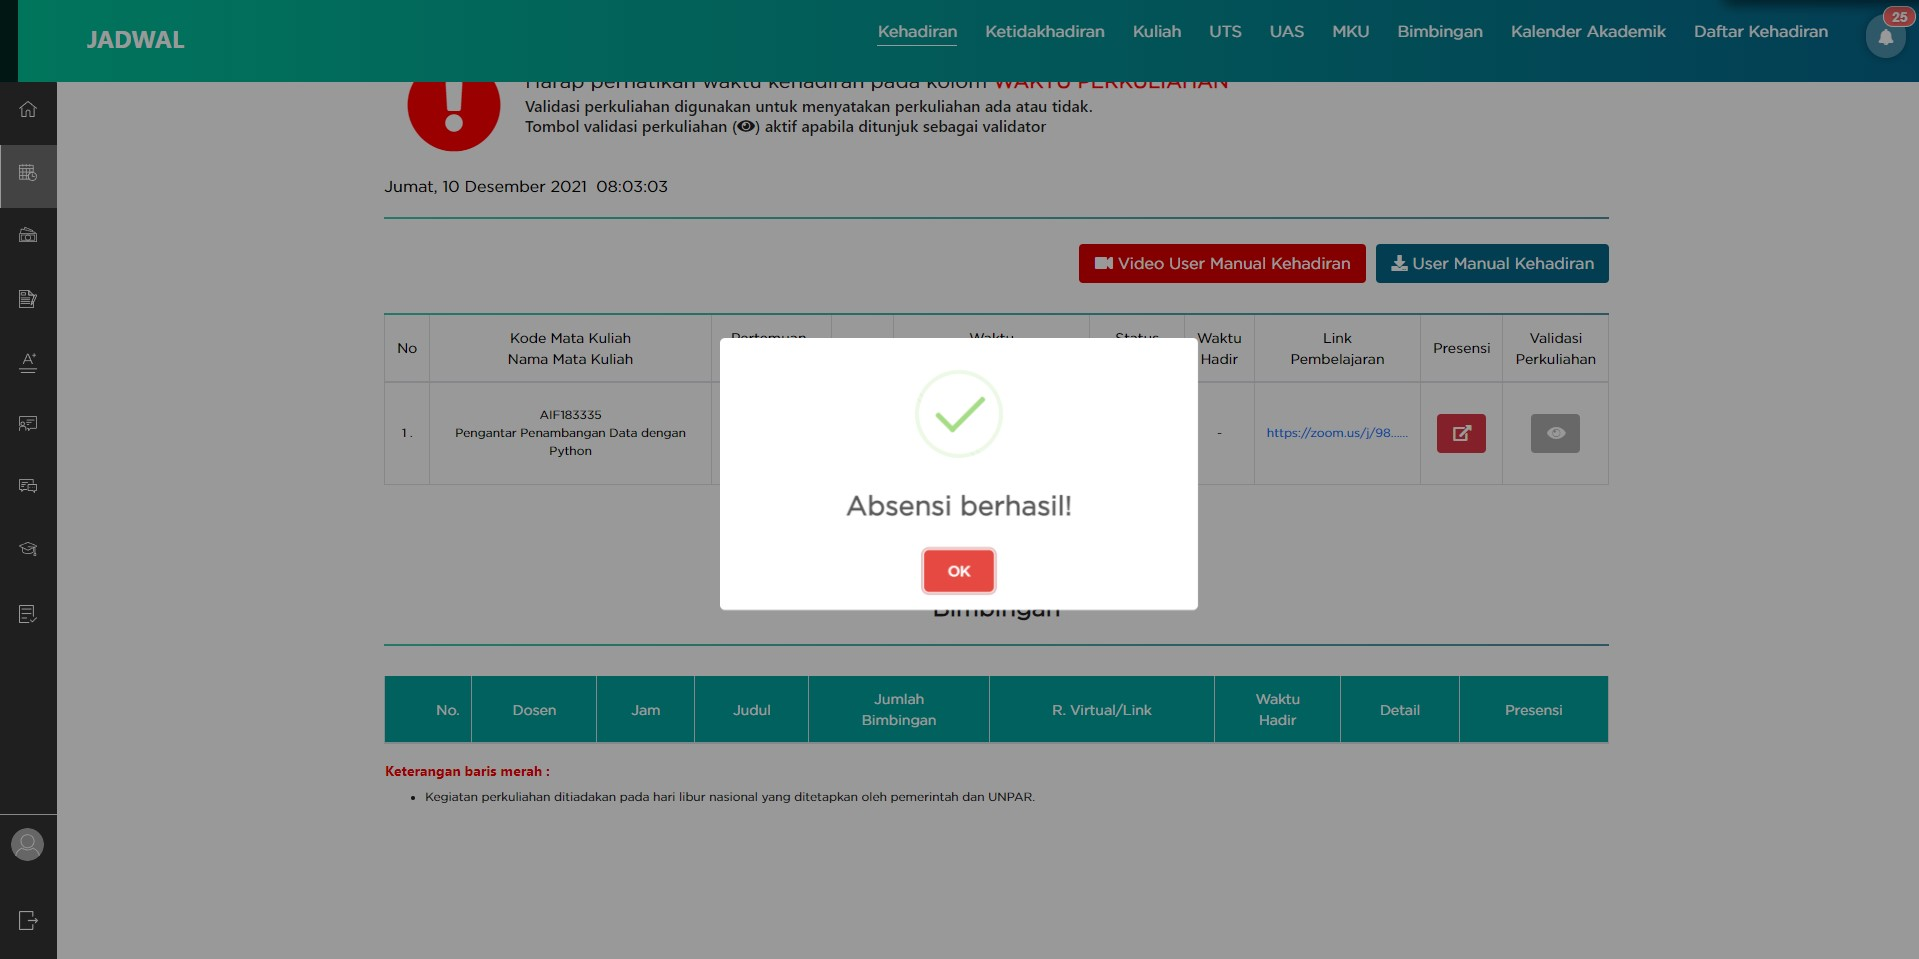
\includegraphics[scale=0.225]{Gambar/berhasilAbsen.jpg}
				\caption{Tampilan Pemberitahuan Absensi Berhasil} 
				\label{fig:berhasil}
			\end{figure}
		\end{enumerate}

		\item \textbf{Membangun program perekaman kehadiran daring otomatis.}\\
		{\bf Status :} Ada sejak rencana kerja skripsi.\\
		{\bf Hasil :} Akan dilakukan pada Skripsi 2.

		\item \textbf{Melakukan pengujian dan eksperimen.}\\
		{\bf Status :} Ada sejak rencana kerja skripsi. \\
		{\bf Hasil :} Akan dilakukan pada Skripsi 2.

		\item \textbf{Menulis dokumen skripsi.} \\
		{\bf Status :} Ada sejak rencana kerja skripsi.\\
		{\bf Hasil :} Bab 1, Bab 2, Bab 3 sudah selesai ditulis, tetapi tidak menutup kemungkinan terjadi perubahan.
		

	\end{enumerate}

\section{Pencapaian Rencana Kerja}
Langkah-langkah kerja yang berhasil diselesaikan dalam Skripsi 1 ini adalah sebagai berikut:
\begin{enumerate}
\item Melakukan studi mengenai Selenium WebDriver. 
\item Mempelajari bahasa pemrograman python.
\item Mempelajari cara menggunakan Selenium.
\item Melakukan survei ke beberapa mahasiswa Teknik Informatika UNPAR dan beberapa dosen Teknik Informatika UNPAR untuk mengetahui berapa lama waktu yang dibutuhkan untuk melakukan absensi secara daring dan luring.
\item Menganalisis web Student Portal UNPAR.
\item Menulis dokumen skripsi Bab 1-3.
\end{enumerate}



\vspace{1cm}
\centering Bandung, \tanggal\\
\vspace{2cm} \nama \\ 
\vspace{1cm}

Menyetujui, \\
\ifdefstring{\jumpemb}{2}{
\vspace{1.5cm}
\begin{centering} Menyetujui,\\ \end{centering} \vspace{0.75cm}
\begin{minipage}[b]{0.45\linewidth}
% \centering Bandung, \makebox[0.5cm]{\hrulefill}/\makebox[0.5cm]{\hrulefill}/2013 \\
\vspace{2cm} Nama: \pembA \\ Pembimbing Utama
\end{minipage} \hspace{0.5cm}
\begin{minipage}[b]{0.45\linewidth}
% \centering Bandung, \makebox[0.5cm]{\hrulefill}/\makebox[0.5cm]{\hrulefill}/2013\\
\vspace{2cm} Nama: \pembB \\ Pembimbing Pendamping
\end{minipage}
\vspace{0.5cm}
}{
% \centering Bandung, \makebox[0.5cm]{\hrulefill}/\makebox[0.5cm]{\hrulefill}/2013\\
\vspace{2cm} Nama: \pembA \\ Pembimbing Tunggal
}
\end{document}

